\documentclass[12pt,a4paper]{report}

\usepackage[a4paper,margin=1in]{geometry}
\usepackage{setspace}
\usepackage{graphicx}
\usepackage{booktabs}
\usepackage{longtable}
\usepackage{array}
\usepackage{xcolor}
\usepackage{hyperref}
\usepackage{titlesec}
\usepackage{fancyhdr}
\usepackage{enumitem}
\usepackage{tikz}
\usepackage{pgfgantt}

\usetikzlibrary{arrows.meta,positioning,shapes.geometric,shapes.misc}

\hypersetup{
  colorlinks=true,
  linkcolor=blue,
  urlcolor=blue,
  citecolor=blue
}

\setstretch{1.3}

% ---- Project metadata ----
\newcommand{\ProjectTitle}{Client Management System (CMS) with Analytics \& Recommendation}
\newcommand{\SubmittedBy}{Bipin Baral and Sudan Tandan}
\newcommand{\ProgramName}{Bachelor in Computer Application (BCA)}
\newcommand{\InstitutionName}{Sagarmatha College of Science and Technology}
\newcommand{\SupervisorName}{Manis Aryal}
\newcommand{\SubmissionDate}{Feb 2026}

\pagestyle{fancy}
\fancyhf{}
\fancyhead[L]{\ProjectTitle}
\fancyhead[R]{\thepage}
\renewcommand{\headrulewidth}{0.4pt}

\begin{document}

% ---------------- Title Page ----------------
\begin{titlepage}
  \centering
  \vspace*{1.0cm}

  {\Large \textbf{\ProjectTitle} \par}
  \vspace{0.4cm}
  {\large \textbf{Project Report} \par}

  \vspace{1.2cm}

  {\large Submitted by \par}
  \vspace{0.2cm}
  {\large \textbf{\SubmittedBy} \par}

  \vspace{0.8cm}
  {\large Program/Department: \textbf{\ProgramName} \par}
  \vspace{0.2cm}
  {\large College/University: \textbf{\InstitutionName} \par}

  \vspace{0.8cm}
  {\large Submitted To (Supervisor): \textbf{\SupervisorName} \par}

  \vfill
  {\large Submission Date: \textbf{\SubmissionDate} \par}
\end{titlepage}

\pagenumbering{roman}

% ---------------- Disclaimer ----------------
\chapter*{Disclaimer}
\addcontentsline{toc}{chapter}{Disclaimer}
I hereby declare that this project report titled \textbf{``Client Management System (CMS) with Analytics \& Recommendation''} is our original work. All sources of information used in this report have been duly acknowledged. This report has not been submitted to any other institution for any academic award.

\vspace{1cm}
\noindent \textbf{Signature:} \rule{6cm}{0.4pt}\\
\textbf{Name:} \SubmittedBy\\
\textbf{Date:} \SubmissionDate

% ---------------- Supervisor’s Recommendation ----------------
\chapter*{Supervisor's Recommendation}
\addcontentsline{toc}{chapter}{Supervisor's Recommendation}
This is to certify that the project report entitled \textbf{``Client Management System (CMS) with Analytics \& Recommendation''} submitted by \textbf{\SubmittedBy} has been prepared under my supervision and is recommended for evaluation.

\vspace{1cm}
\noindent \textbf{Supervisor:} \SupervisorName\\
\textbf{Signature:} \rule{6cm}{0.4pt}\\
\textbf{Date:} \SubmissionDate

% ---------------- Certificate of Approval ----------------
\chapter*{Certificate of Approval}
\addcontentsline{toc}{chapter}{Certificate of Approval}
This project report entitled \textbf{``Client Management System (CMS) with Analytics \& Recommendation''} submitted by \textbf{\SubmittedBy} is approved in partial fulfillment of the requirement for the degree/program \textbf{\ProgramName}.

\vspace{0.6cm}
\begin{longtable}{@{}p{4.2cm}p{5.0cm}p{3.5cm}p{2.2cm}@{}}
\toprule
\textbf{Committee/Authority} & \textbf{Name} & \textbf{Signature} & \textbf{Date} \\
\midrule
Supervisor & \SupervisorName &  &  \\
Examiner & \rule{4.5cm}{0.4pt} &  &  \\
Head/Coordinator & \rule{4.5cm}{0.4pt} &  &  \\
\bottomrule
\end{longtable}

% ---------------- Acknowledgement ----------------
\chapter*{Acknowledgement}
\addcontentsline{toc}{chapter}{Acknowledgement}
We would like to express our sincere gratitude to our supervisor \textbf{\SupervisorName} for guidance and continuous support. We also thank our department, friends, and family for their encouragement during the completion of this project.

% ---------------- Abstract ----------------
\chapter*{Abstract}
\addcontentsline{toc}{chapter}{Abstract}
The \textbf{Client Management System (CMS)} is a web-based application designed to manage client profiles, workouts, payments, and notes for service providers such as trainers/freelancers, while also offering administrative insights through analytics and activity logs. The system consists of a \textbf{Next.js (App Router) frontend} and a \textbf{Node.js/Express backend} connected to \textbf{MongoDB} using \textbf{Mongoose}. Security is handled through \textbf{JWT-based authentication}, password hashing using \textbf{bcrypt}, request validation using \textbf{express-validator}, and protection against abuse through \textbf{rate limiting}. Key capabilities include client CRUD operations with fuzzy search, workout management with rating, payment tracking with overdue/due-soon analytics, note-taking with tagging and completion, and dashboard analytics including trends and forecasting. Localization support includes \textbf{Nepal-specific phone validation} and default currency handling (NPR). This report presents the problem context, objectives, system analysis, design, implementation, and testing outcomes, along with future enhancement recommendations.

% ---------------- TOC / Lists ----------------
\tableofcontents
\listoffigures
\listoftables

% ---------------- Abbreviations ----------------
\chapter*{Abbreviations}
\addcontentsline{toc}{chapter}{Abbreviations}
\begin{longtable}{@{}p{2.5cm}p{11cm}@{}}
\toprule
\textbf{Term} & \textbf{Meaning}\\
\midrule
API & Application Programming Interface\\
CMS & Client Management System\\
CRUD & Create, Read, Update, Delete\\
DFD & Data Flow Diagram\\
ER & Entity Relationship\\
JWT & JSON Web Token\\
RBAC & Role-Based Access Control\\
REST & Representational State Transfer\\
TTL & Time To Live (automatic expiry)\\
UI/UX & User Interface / User Experience\\
\bottomrule
\end{longtable}

\clearpage
\pagenumbering{arabic}

% ============================================================
\chapter{Introduction}
\section{Introduction}
Client-oriented businesses (e.g., training, freelancing, service providers) require organized handling of client data, service history, payments, and communications. Manual processes using spreadsheets and scattered notes often lead to inconsistency, missed follow-ups, and delayed payments. The proposed \textbf{Client Management System (CMS)} provides a centralized and secure platform to manage clients, create workouts/programs, maintain notes, track payments (including overdue cases), and derive insights from analytics.

\section{Problem Statement}
Existing client handling methods commonly face the following issues:
\begin{itemize}[leftmargin=*]
  \item Fragmented records (client info, workouts, and payments stored in different places)
  \item Lack of reliable overdue payment tracking and reminders
  \item Limited insight into growth, revenue trends, and client activity
  \item Inefficient search when client lists grow large (typos and partial matches)
  \item Weak security practices in ad-hoc systems (no authentication, no logging)
\end{itemize}

\section{Objectives}
\subsection*{General Objective}
To develop a secure, web-based client management system with analytics and recommendation features.

\subsection*{Specific Objectives}
\begin{itemize}[leftmargin=*]
  \item Provide authentication using JWT and secure password hashing
  \item Manage client profiles with advanced search and filtering
  \item Manage workouts and support rating to improve recommendations
  \item Track payments and detect overdue/due-soon payments with analytics
  \item Store structured notes with tags, priority, and completion workflow
  \item Provide analytics dashboards (client activity, revenue trends, logs)
  \item Maintain activity logs for auditing and monitoring
  \item Support Nepal localization (phone validation and NPR default currency)
\end{itemize}

\section{Scope}
The scope of this project includes:
\begin{itemize}[leftmargin=*]
  \item \textbf{Frontend (Next.js):} Public pages, authentication pages, dashboard pages, admin panel UI, reusable UI components.
  \item \textbf{Backend (Express):} REST API endpoints for authentication, clients, workouts, payments, notes, analytics, and countries.
  \item \textbf{Database (MongoDB):} Persistent storage for users, clients, workouts, payments, notes, and activity logs.
  \item \textbf{Algorithms:} Fuzzy search, activity scoring, KNN-based similarity/recommendations, priority queue for overdue payments, trend forecasting.
\end{itemize}
Out of scope (current version): real-time messaging, CI/CD deployment, third-party payment gateway integration, and multi-tenant organization accounts.

\section{Limitations}
\begin{itemize}[leftmargin=*]
  \item The frontend includes static/mock UI data for many dashboards; full API integration can be extended.
  \item In-memory rate limit store is used (recommended: Redis in production).
  \item Admin authentication in UI is represented as static credentials in the UI summary; production-grade admin auth should be backend-driven.
  \item Recommendation and forecasting quality depends on available data volume.
\end{itemize}

\section{Development Methodology}
This project follows the \textbf{Waterfall Model} because requirements and module boundaries (auth, clients, payments, workouts, notes, analytics) are clear and can be implemented in sequential phases:
\begin{enumerate}[leftmargin=*]
  \item Requirements gathering and analysis
  \item System design (architecture + database + interface design)
  \item Implementation (backend and frontend modules)
  \item Integration and testing
  \item Deployment (local environment) and documentation
\end{enumerate}

\section{Report Organization}
\begin{table}[h]
\centering
\caption{Report Organization}
\begin{tabular}{@{}p{1.2cm}p{4.0cm}p{7.8cm}@{}}
\toprule
\textbf{Ch.} & \textbf{Title} & \textbf{Description} \\
\midrule
1 & Introduction & Problem, objectives, scope, methodology \\
2 & Background \& Literature Review & Related systems and supporting technologies \\
3 & System Analysis & Requirements, feasibility, DFD, ER, schedule \\
4 & System Design & Architecture, design approach, flowcharts \\
5 & Implementation \& Testing & Environment, module implementation, tests \\
6 & Conclusion \& Future Work & Outcomes, improvements \\
7 & Appendix & Screenshots, configuration samples \\
8 & References & Books, papers, documentation links \\
\bottomrule
\end{tabular}
\end{table}

% ============================================================
\chapter{Background Study and Literature Review}
\section{Background Study}
Client management platforms (CRM-like systems) are widely used to store client details and track engagements. In fitness and service contexts, additional domain needs include program/workout assignment, progress notes, and recurring payments. Modern web systems typically use a frontend framework (React/Next.js) connected to a backend API (Node.js/Express) and a database (MongoDB/SQL).

\section{Literature Review}
This project is influenced by best practices and concepts from:
\begin{itemize}[leftmargin=*]
  \item \textbf{JWT Authentication:} Stateless session handling for APIs; tokens passed via \texttt{Authorization: Bearer <token>}.
  \item \textbf{Password Hashing (bcrypt):} One-way hashing and salting of passwords to prevent plaintext storage.
  \item \textbf{MongoDB + Mongoose:} Flexible document storage for evolving requirements, schema modeling, and indexing.
  \item \textbf{REST API Design:} Clear endpoints and status codes; pagination/filtering for large datasets.
  \item \textbf{Fuzzy Search:} Improves UX by allowing typo-tolerant search.
  \item \textbf{KNN-based similarity:} Similarity-based recommendations (e.g., similar clients; workout suggestions).
  \item \textbf{Forecasting:} Linear regression and moving average smoothing to interpret revenue trends.
  \item \textbf{Rate Limiting:} Limits requests per IP and endpoint type to reduce abuse.
\end{itemize}

% ============================================================
\chapter{System Analysis}
\section{Requirement Analysis}
The system requirements were derived from the core problems: secure login, managing client lifecycle, tracking workouts, tracking payments and due dates, note-taking, and analytics reporting.

\subsection{Functional Requirements}
\begin{table}[h]
\centering
\caption{Functional Requirements}
\begin{tabular}{@{}p{1.5cm}p{4.0cm}p{8.0cm}@{}}
\toprule
\textbf{ID} & \textbf{Requirement} & \textbf{Description} \\
\midrule
FR-01 & User registration & Register a user with name/email/password \\
FR-02 & User login & Login and receive JWT token \\
FR-03 & Client management & Add/update/view/soft-delete clients \\
FR-04 & Client search & Fuzzy search clients by name/email/phone \\
FR-05 & Inactive clients & Identify clients inactive for 7+ days \\
FR-06 & Workout management & CRUD workouts; filter/search workouts \\
FR-07 & Workout rating & Rate workouts (1--5) and store metrics \\
FR-08 & Recommendations & Recommend workouts and find similar clients \\
FR-09 & Payment management & Create/update/view payments with invoices \\
FR-10 & Overdue detection & List overdue payments and prioritize them \\
FR-11 & Notes management & CRUD notes with tags/priority/completion \\
FR-12 & Analytics dashboard & Provide aggregated statistics and trends \\
FR-13 & Activity logs & Record and query activity logs for auditing \\
FR-14 & Localization & Nepal phone validation; default currency NPR \\
\bottomrule
\end{tabular}
\end{table}

\section{Feasibility Study}
\subsection{Technical Feasibility}
Node.js/Express, Next.js, and MongoDB are stable and widely supported. JWT and bcrypt provide standard security, while indexing and pagination support performance at scale.

\subsection{Operational Feasibility}
The system centralizes client records, payments, notes, and workouts, improving efficiency and reducing missed follow-ups. Dashboards and analytics assist decision making.

\subsection{Economic Feasibility}
The system is cost-effective due to open-source tooling and local deployment capability. Cloud deployment can be added later as needed.

\begin{table}[h]
\centering
\caption{Feasibility Study Summary}
\begin{tabular}{@{}p{4.2cm}p{2.6cm}p{6.8cm}@{}}
\toprule
\textbf{Feasibility Type} & \textbf{Result} & \textbf{Notes}\\
\midrule
Technical & Feasible & Stable ecosystem; modular design\\
Operational & Feasible & Improves workflow; reduces errors\\
Economic & Feasible & Low cost; open-source stack\\
\bottomrule
\end{tabular}
\end{table}

\section{Schedule (Gantt Chart)}
\begin{figure}[h]
\centering
\caption{Gantt Chart (Sample Schedule)}
\begin{ganttchart}[
  hgrid,
  vgrid,
  time slot format=isodate-yearmonth,
  compress calendar,
  title/.append style={fill=gray!10},
  bar/.append style={fill=blue!30},
  bar height=0.6,
  group/.append style={fill=blue!15},
]{2026-01}{2026-02}
  \gantttitlecalendar{year, month} \\
  \ganttgroup{Analysis \& Design}{2026-01}{2026-01} \\
  \ganttbar{Requirements}{2026-01}{2026-01} \\
  \ganttbar{Architecture/DB Design}{2026-01}{2026-01} \\
  \ganttgroup{Implementation}{2026-01}{2026-02} \\
  \ganttbar{Backend (Auth + Core APIs)}{2026-01}{2026-02} \\
  \ganttbar{Algorithms + Analytics}{2026-01}{2026-02} \\
  \ganttbar{Frontend UI}{2026-01}{2026-02} \\
  \ganttbar{Integration}{2026-02}{2026-02} \\
  \ganttgroup{Testing \& Documentation}{2026-02}{2026-02} \\
  \ganttbar{Testing}{2026-02}{2026-02} \\
  \ganttbar{Report Writing}{2026-02}{2026-02} \\
\end{ganttchart}
\end{figure}

\section{Data Flow Diagram (DFD)}
\subsection{DFD Level 0 (Context Diagram)}
\begin{figure}[h]
\centering
\caption{DFD Level 0 (Context Diagram)}
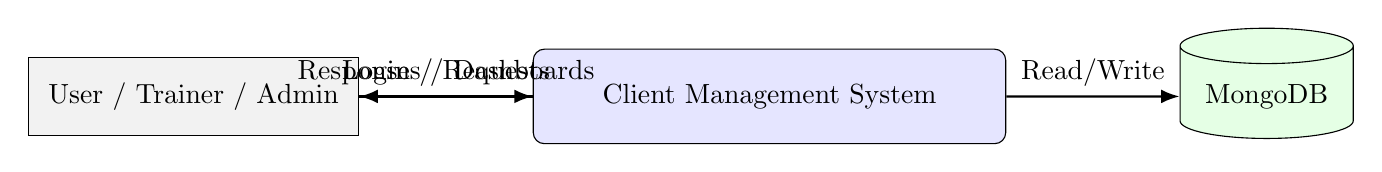
\begin{tikzpicture}[
  node distance=2.2cm,
  proc/.style={draw,rounded corners,minimum width=6.0cm,minimum height=1.2cm,fill=blue!10},
  ext/.style={draw,minimum width=4.2cm,minimum height=1.0cm,fill=gray!10},
  db/.style={draw,cylinder,shape border rotate=90,aspect=0.25,minimum height=1.4cm,minimum width=2.2cm,fill=green!10},
  arr/.style={-Latex,thick}
]
  \node[ext] (u) {User / Trainer / Admin};
  \node[proc, right=of u] (s) {Client Management System};
  \node[db, right=of s] (db) {MongoDB};

  \draw[arr] (u) -- node[above]{Login / Requests} (s);
  \draw[arr] (s) -- node[above]{Responses / Dashboards} (u);
  \draw[arr] (s) -- node[above]{Read/Write} (db);
\end{tikzpicture}
\end{figure}

\subsection{DFD Level 1 (Main Processes)}
\begin{figure}[p]
\centering
\caption{DFD Level 1 (Main Processes)}
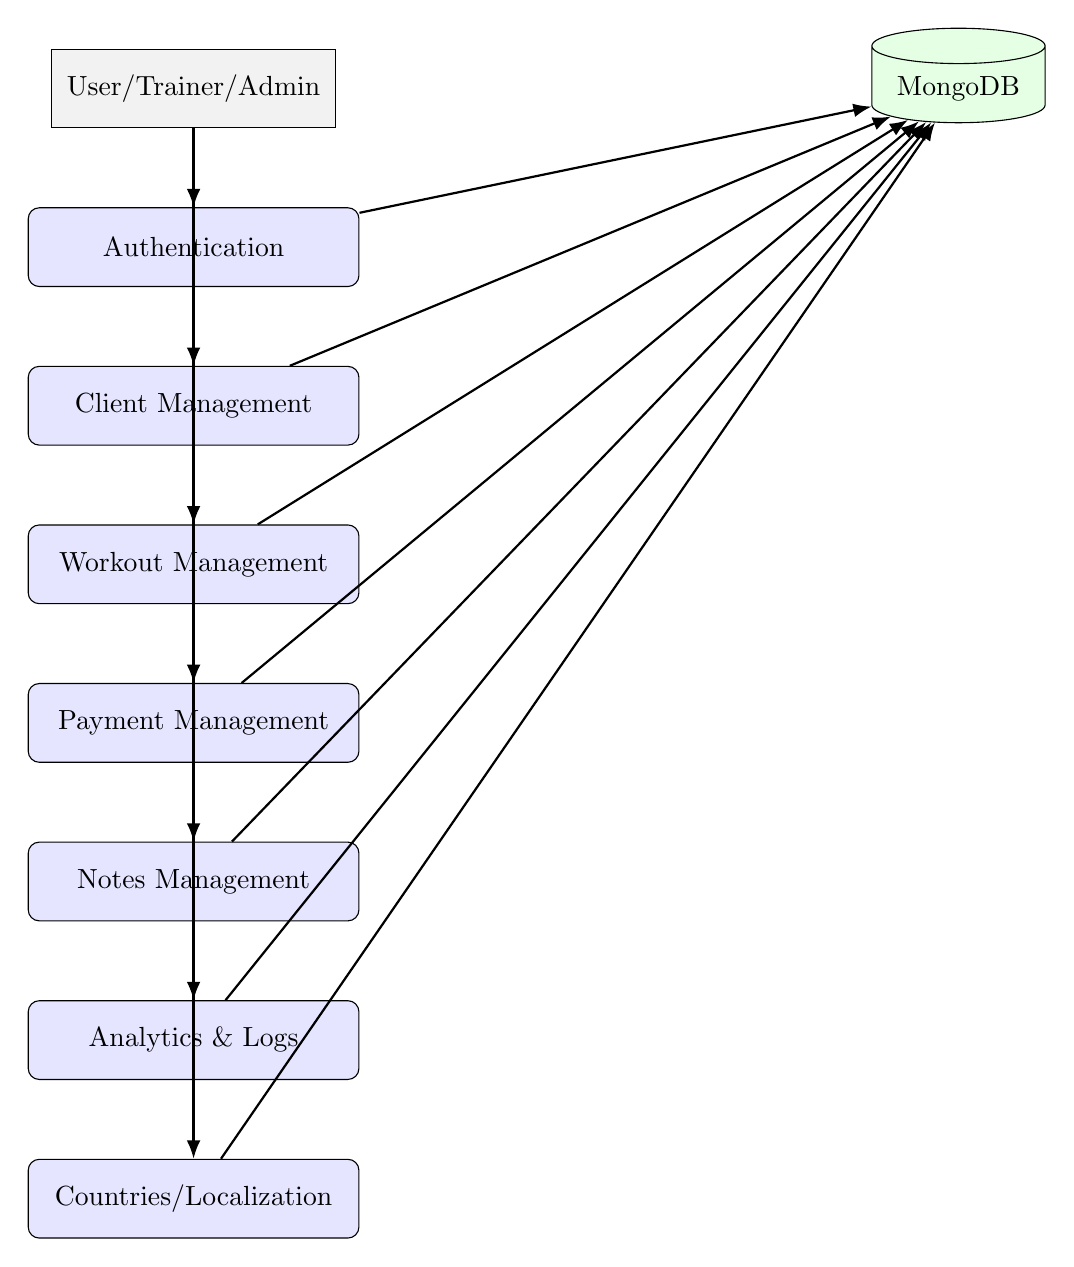
\begin{tikzpicture}[
  node distance=1.0cm and 1.2cm,
  ext/.style={draw,minimum width=3.6cm,minimum height=1.0cm,fill=gray!10},
  proc/.style={draw,rounded corners,minimum width=4.2cm,minimum height=1.0cm,fill=blue!10},
  db/.style={draw,cylinder,shape border rotate=90,aspect=0.25,minimum height=1.2cm,minimum width=2.2cm,fill=green!10},
  arr/.style={-Latex,thick}
]
  \node[ext] (u) {User/Trainer/Admin};
  \node[db, right=6.8cm of u] (db) {MongoDB};

  \node[proc, below=of u] (p1) {Authentication};
  \node[proc, below=of p1] (p2) {Client Management};
  \node[proc, below=of p2] (p3) {Workout Management};
  \node[proc, below=of p3] (p4) {Payment Management};
  \node[proc, below=of p4] (p5) {Notes Management};
  \node[proc, below=of p5] (p6) {Analytics \& Logs};
  \node[proc, below=of p6] (p7) {Countries/Localization};

  \foreach \p in {p1,p2,p3,p4,p5,p6,p7} {
    \draw[arr] (u) -- (\p);
    \draw[arr] (\p) -- (db);
  }
\end{tikzpicture}
\end{figure}

\section{Entity Relationship (ER) Diagram}
\begin{figure}[p]
\centering
\caption{ER Diagram (Logical Data Model)}
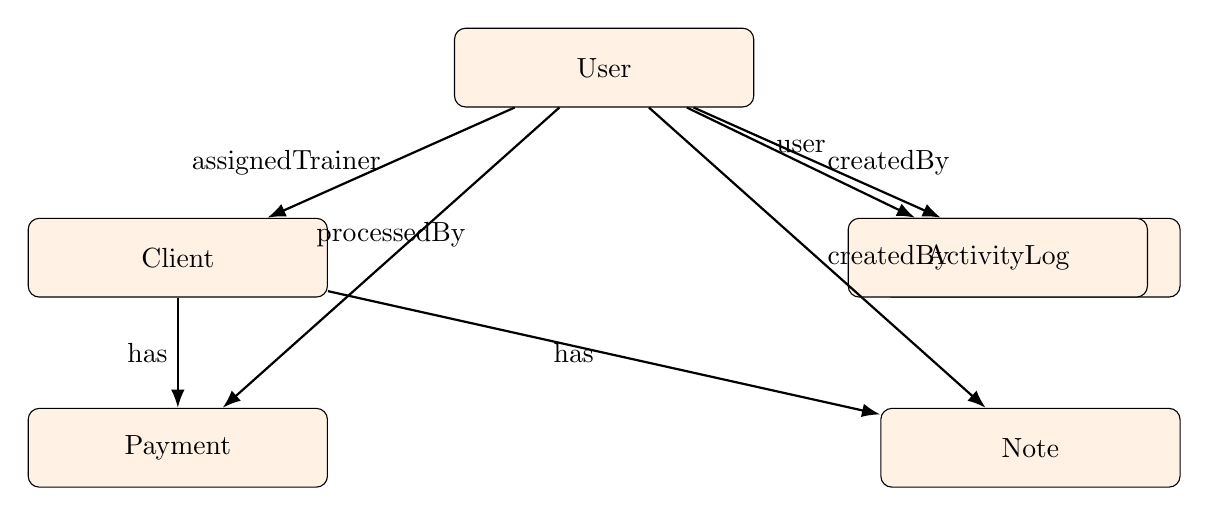
\begin{tikzpicture}[
  node distance=1.4cm and 1.6cm,
  ent/.style={draw,rounded corners,fill=orange!10,minimum width=3.8cm,minimum height=1.0cm,align=center},
  arr/.style={-Latex,thick}
]
  \node[ent] (user) {User};
  \node[ent, below left=of user] (client) {Client};
  \node[ent, below right=of user] (workout) {Workout};
  \node[ent, below=of client] (payment) {Payment};
  \node[ent, below=of workout] (note) {Note};
  \node[ent, below=of user, xshift=5.0cm] (log) {ActivityLog};

  \draw[arr] (user) -- node[left]{assignedTrainer} (client);
  \draw[arr] (user) -- node[right]{createdBy} (workout);
  \draw[arr] (user) -- node[right]{createdBy} (note);
  \draw[arr] (user) -- node[above]{processedBy} (payment);
  \draw[arr] (user) -- node[above]{user} (log);

  \draw[arr] (client) -- node[left]{has} (payment);
  \draw[arr] (client) -- node[left]{has} (note);
\end{tikzpicture}
\end{figure}

% ============================================================
\chapter{System Design}
\section{System Design Overview}
The system follows a \textbf{three-tier architecture}:
\begin{itemize}[leftmargin=*]
  \item \textbf{Presentation Layer:} Next.js frontend (UI pages, components, navigation)
  \item \textbf{Application Layer:} Express backend (business logic, security, algorithms)
  \item \textbf{Data Layer:} MongoDB (persistent data storage, indexes, analytics)
\end{itemize}

\section{Methodology of the Proposed System}
The proposed system uses REST APIs for communication between frontend and backend, JWT-based stateless authentication, validation middleware for data integrity, rate limiting to prevent brute-force and abuse, and modular separation of concerns (routes/controllers/models/middleware).

\section{Flowcharts}
\subsection{Authentication Flow (Login/Register)}
\begin{figure}[h]
\centering
\caption{Authentication Flow}
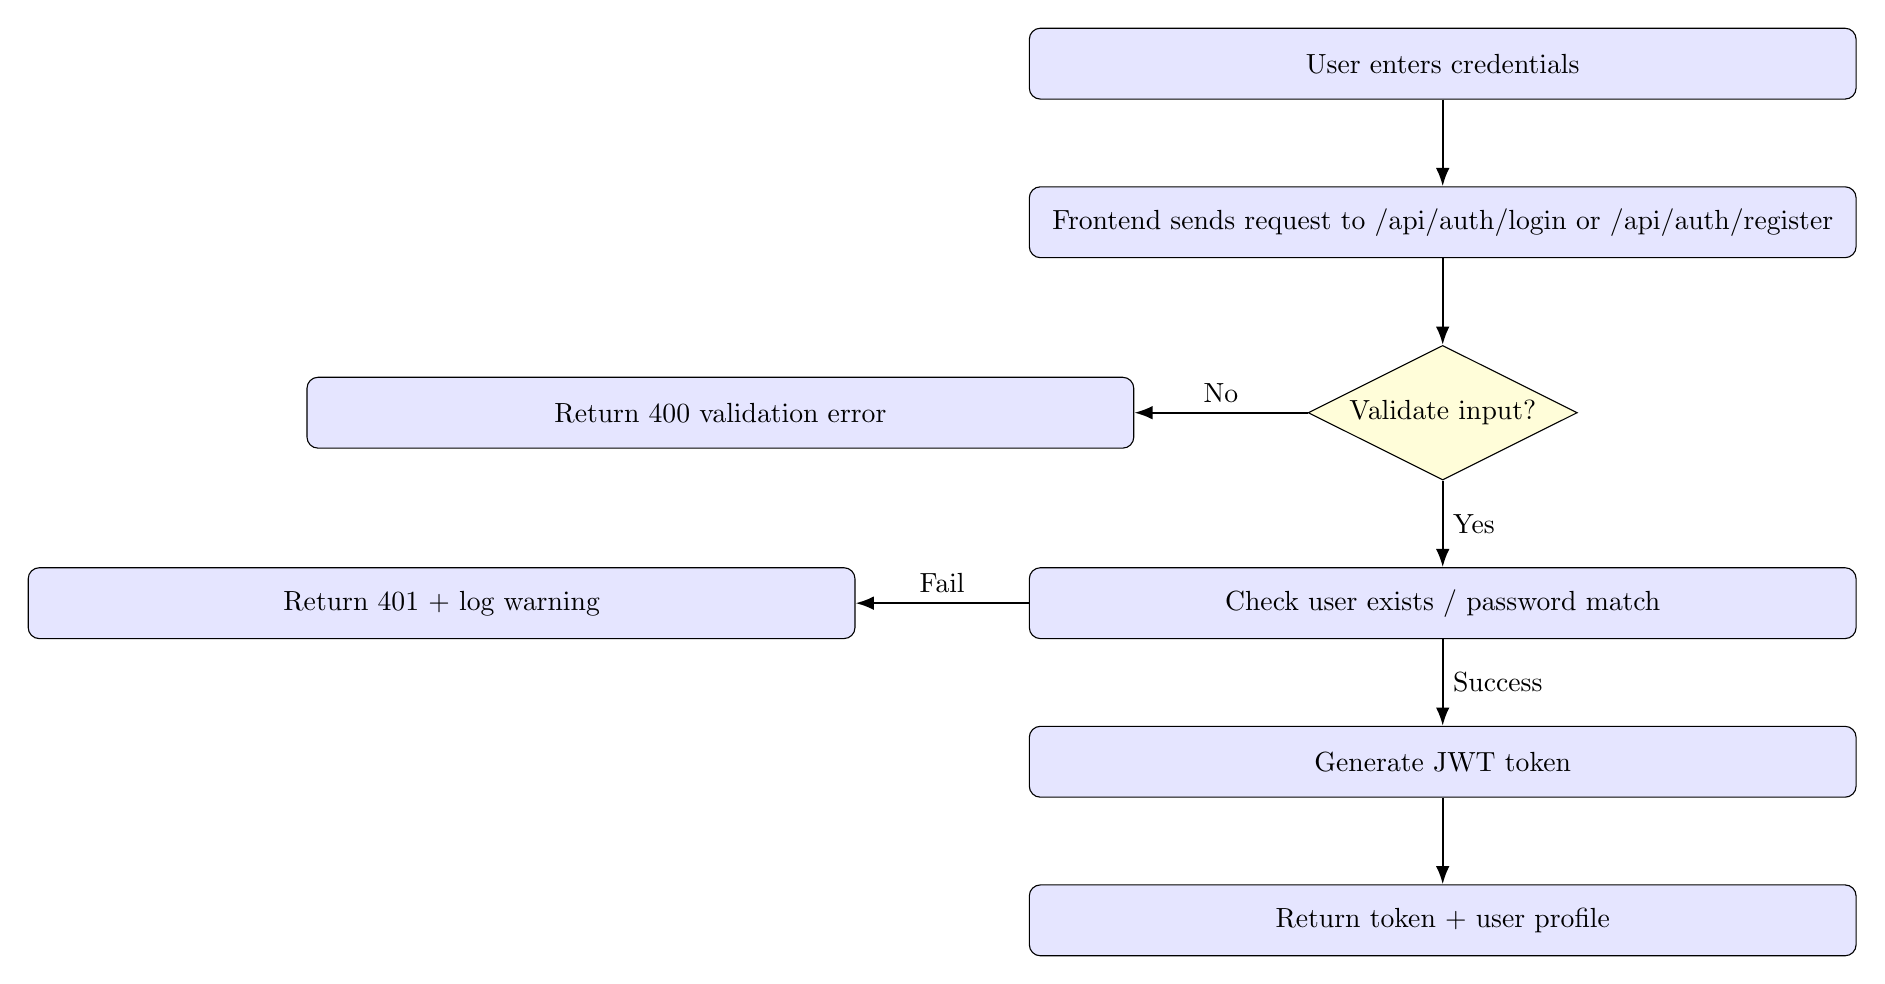
\begin{tikzpicture}[
  node distance=1.1cm,
  box/.style={draw,rounded corners,fill=blue!10,minimum width=10.5cm,minimum height=0.9cm,align=center},
  decision/.style={draw,diamond,aspect=2,fill=yellow!15,align=center,inner sep=2pt},
  arr/.style={-Latex,thick}
]
  \node[box] (a) {User enters credentials};
  \node[box, below=of a] (b) {Frontend sends request to /api/auth/login or /api/auth/register};
  \node[decision, below=of b] (c) {Validate input?};
  \node[box, left=2.2cm of c] (d) {Return 400 validation error};
  \node[box, below=of c] (e) {Check user exists / password match};
  \node[box, left=2.2cm of e] (f) {Return 401 + log warning};
  \node[box, below=of e] (g) {Generate JWT token};
  \node[box, below=of g] (h) {Return token + user profile};

  \draw[arr] (a) -- (b);
  \draw[arr] (b) -- (c);
  \draw[arr] (c) -- node[above]{No} (d);
  \draw[arr] (c) -- node[right]{Yes} (e);
  \draw[arr] (e) -- node[above]{Fail} (f);
  \draw[arr] (e) -- node[right]{Success} (g);
  \draw[arr] (g) -- (h);
\end{tikzpicture}
\end{figure}

\subsection{Client Management Flow}
\begin{figure}[p]
\centering
\caption{Client Management Flowchart}
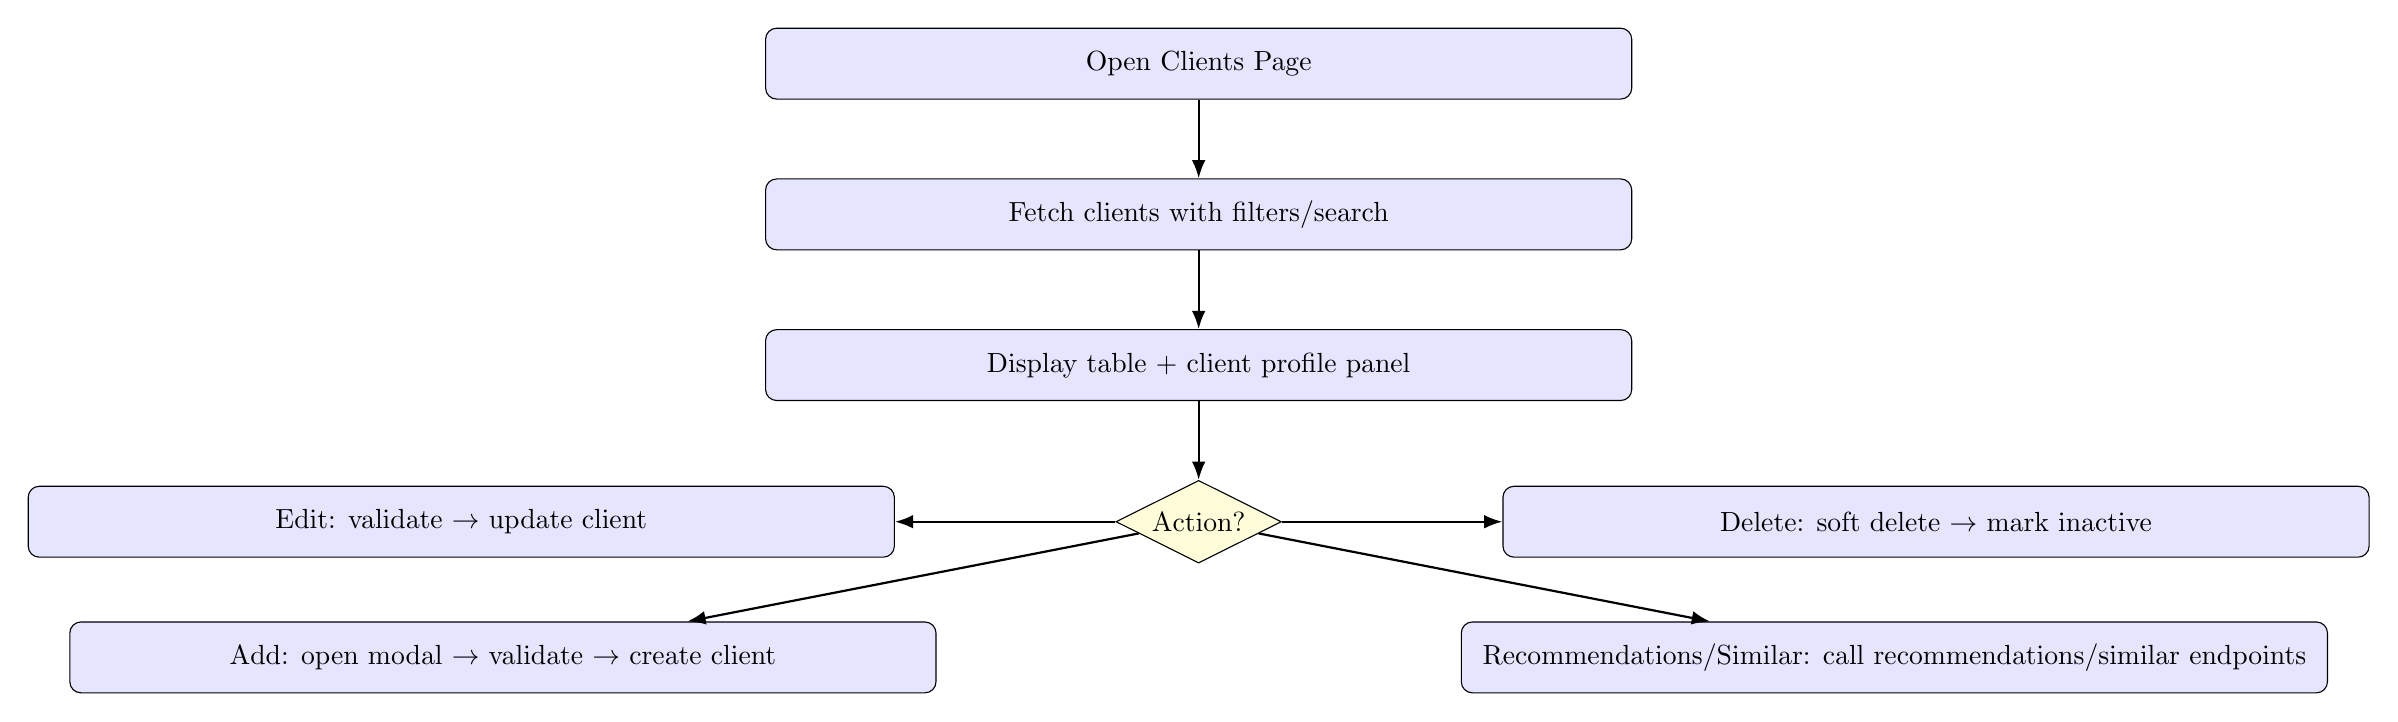
\begin{tikzpicture}[
  node distance=1.0cm,
  box/.style={draw,rounded corners,fill=blue!10,minimum width=11cm,minimum height=0.9cm,align=center},
  decision/.style={draw,diamond,aspect=2,fill=yellow!15,align=center,inner sep=2pt},
  arr/.style={-Latex,thick}
]
  \node[box] (a) {Open Clients Page};
  \node[box, below=of a] (b) {Fetch clients with filters/search};
  \node[box, below=of b] (c) {Display table + client profile panel};
  \node[decision, below=of c] (d) {Action?};

  \node[box, below left=1.0cm and 2.8cm of d] (e) {Add: open modal \(\rightarrow\) validate \(\rightarrow\) create client};
  \node[box, left=2.8cm of d] (f) {Edit: validate \(\rightarrow\) update client};
  \node[box, right=2.8cm of d] (g) {Delete: soft delete \(\rightarrow\) mark inactive};
  \node[box, below right=1.0cm and 2.8cm of d] (h) {Recommendations/Similar: call recommendations/similar endpoints};

  \draw[arr] (a) -- (b);
  \draw[arr] (b) -- (c);
  \draw[arr] (c) -- (d);
  \draw[arr] (d) -- (e);
  \draw[arr] (d) -- (f);
  \draw[arr] (d) -- (g);
  \draw[arr] (d) -- (h);
\end{tikzpicture}
\end{figure}

\subsection{Payment Overdue Detection Flow}
\begin{figure}[h]
\centering
\caption{Payment Overdue Detection Flow}
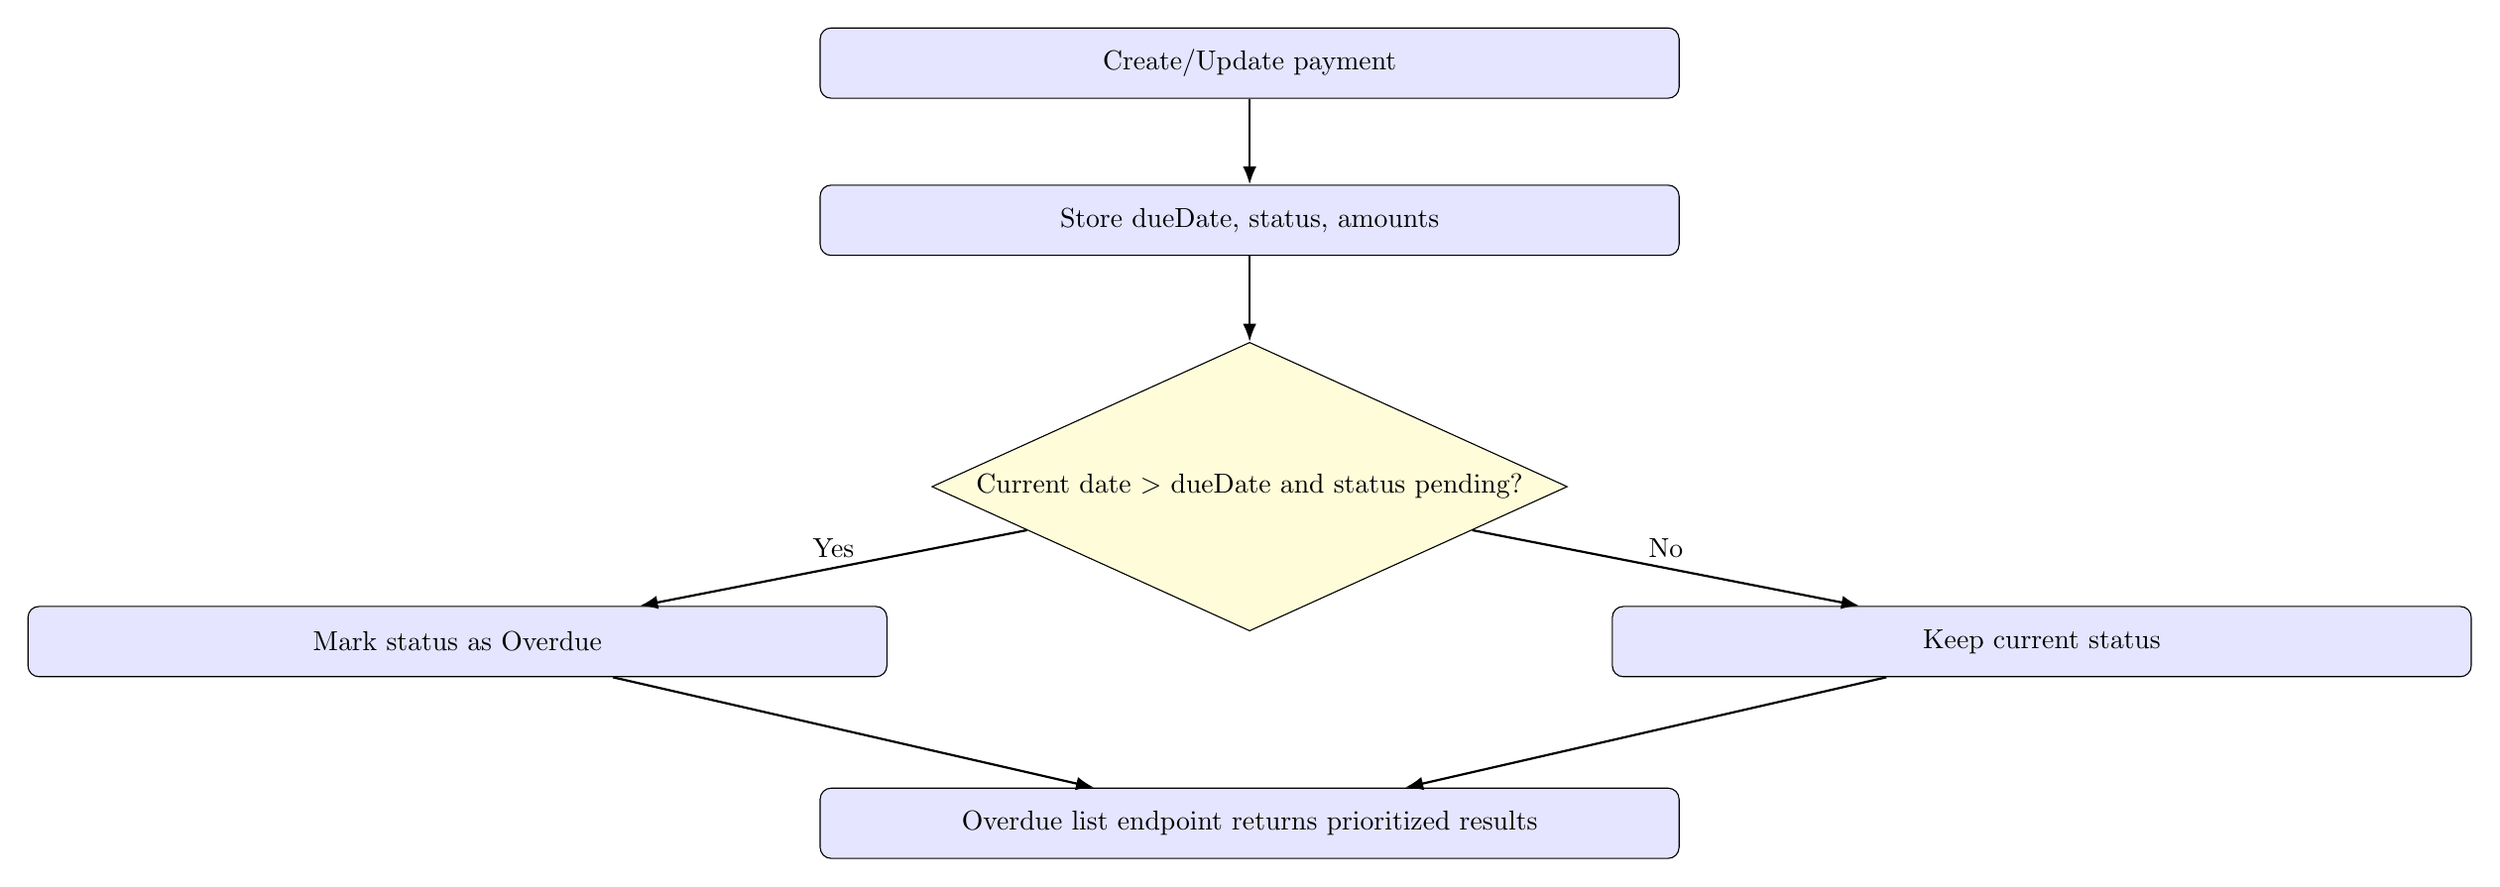
\begin{tikzpicture}[
  node distance=1.1cm,
  box/.style={draw,rounded corners,fill=blue!10,minimum width=11cm,minimum height=0.9cm,align=center},
  decision/.style={draw,diamond,aspect=2.2,fill=yellow!15,align=center,inner sep=2pt},
  arr/.style={-Latex,thick}
]
  \node[box] (a) {Create/Update payment};
  \node[box, below=of a] (b) {Store dueDate, status, amounts};
  \node[decision, below=of b] (c) {Current date \(>\) dueDate and status pending?};
  \node[box, below left=0.6cm and 2.6cm of c] (d) {Mark status as Overdue};
  \node[box, below right=0.6cm and 2.6cm of c] (e) {Keep current status};
  \node[box, below=2.0cm of c] (f) {Overdue list endpoint returns prioritized results};

  \draw[arr] (a) -- (b);
  \draw[arr] (b) -- (c);
  \draw[arr] (c) -- node[above]{Yes} (d);
  \draw[arr] (c) -- node[above]{No} (e);
  \draw[arr] (d) -- (f);
  \draw[arr] (e) -- (f);
\end{tikzpicture}
\end{figure}

\section{Working Mechanism and Tools}
\subsection*{Frontend Tools}
Next.js (App Router), React, TypeScript, TailwindCSS v4, Radix UI primitives, Lucide icons, Chart.js and react-chartjs-2.

\subsection*{Backend Tools}
Node.js + Express, MongoDB + Mongoose, JWT, bcryptjs, express-validator, express-rate-limit, Fuse.js (fuzzy search), node-cron (available for scheduled tasks).

% ============================================================
\chapter{Implementation and Testing}
\section{System Implementation}
\subsection{Development Environment Setup}
\textbf{Backend:} \texttt{backend/} \\
Run: \texttt{npm install}, create \texttt{.env} from \texttt{.env.example}, then \texttt{npm run dev}. \\
\textbf{Frontend:} \texttt{frontend/} \\
Run: \texttt{npm install} or \texttt{pnpm install}, then \texttt{pnpm dev} or \texttt{npm run dev}.

\subsection{Admin Module Development}
The frontend includes an admin panel UI under routes such as: \texttt{/admin}, \texttt{/admin/users}, \texttt{/admin/reports}, \texttt{/admin/logs}, \texttt{/admin/settings}.

\subsection{Client Module Development}
Protected backend endpoints include: \texttt{GET/POST /api/clients}, \texttt{GET/PUT/DELETE /api/clients/:id}, \texttt{GET /api/clients/inactive}, \texttt{GET /api/clients/:id/recommendations}, \texttt{GET /api/clients/:id/similar}.

\subsection{Database Design and Integration}
MongoDB collections and relationships are modeled using Mongoose:
\begin{itemize}[leftmargin=*]
  \item \texttt{Client}: profile + fitness info + activity metrics (BMI/activity score)
  \item \texttt{Workout}: workout programs + rating/popularity metrics + creator reference
  \item \texttt{Payment}: invoices + overdue logic + analytics-friendly fields
  \item \texttt{Note}: tagged notes per client + completion workflow
  \item \texttt{ActivityLog}: audit logs with TTL (90 days)
\end{itemize}

\subsection{System Integration}
Integration is performed using REST API calls:
\begin{itemize}[leftmargin=*]
  \item JWT passed in request header: \texttt{Authorization: Bearer <token>}
  \item Backend middleware verifies token and attaches user to the request
\end{itemize}

\section{Testing}
\subsection{Unit Testing (Conceptual)}
Unit tests focus on validation rules, model methods (activity score, invoice generation), and algorithm utilities (fuzzy search, similarity scoring, forecasting).

\subsection{Integration Testing}
Integration testing can be performed using Postman/Thunder Client:
\begin{itemize}[leftmargin=*]
  \item Register \(\rightarrow\) Login \(\rightarrow\) access protected endpoints
  \item Create Client \(\rightarrow\) Create Payment \(\rightarrow\) query overdue/due-soon
  \item Create Workout \(\rightarrow\) Rate Workout \(\rightarrow\) verify rating metrics
  \item Create Note \(\rightarrow\) mark complete \(\rightarrow\) verify state change
\end{itemize}

\begin{table}[h]
\centering
\caption{Sample Test Cases}
\begin{tabular}{@{}p{1.4cm}p{4.0cm}p{5.0cm}p{4.2cm}@{}}
\toprule
\textbf{Test ID} & \textbf{Scenario} & \textbf{Input} & \textbf{Expected Output} \\
\midrule
TC-01 & Register user & Valid name/email/password & 201 + JWT token \\
TC-02 & Login user & Correct credentials & 200 + JWT token \\
TC-03 & Create client & Valid Nepal phone (98xxxxxxxx) & 201 created \\
TC-04 & Invalid phone & 9601234567 & 400 validation error \\
TC-05 & Overdue payment & dueDate $<$ today & status becomes Overdue \\
TC-06 & Get overdue payments & GET /payments/overdue & prioritized list \\
\bottomrule
\end{tabular}
\end{table}

% ============================================================
\chapter{Conclusion and Future Recommendation}
\section{Conclusion}
The Client Management System delivers a structured solution for managing client data, workouts, payments, and notes, backed by a secure REST API. JWT authentication, validation, activity logging, and rate limiting improve security and reliability. Analytics endpoints and implemented algorithms (fuzzy search, activity scoring, recommendations, forecasting) enhance decision-making and follow-up. Localization support for Nepal makes the system suitable for local use cases.

\section{Future Recommendations}
\begin{itemize}[leftmargin=*]
  \item Full frontend-to-backend integration across all pages (replace mock data)
  \item Use httpOnly cookies and refresh tokens for improved auth security
  \item Add a role field to User and enforce RBAC for admin endpoints
  \item Add file uploads (profile images, attachments) using cloud storage
  \item Add notifications (email/SMS) for overdue payments and reminders
  \item Add CI/CD pipeline and production deployment
  \item Add automated testing (Jest/Supertest) and API contract tests
  \item Add caching for analytics endpoints (Redis) for performance
\end{itemize}

% ============================================================
\appendix
\chapter{Appendix}
\section{System Screenshots}
Place your screenshots in \texttt{figures/} and replace the placeholders below with \texttt{\textbackslash includegraphics}.

\begin{figure}[h]
\centering
\fbox{\parbox{0.92\textwidth}{\centering \vspace{2.2cm}Screenshot Placeholder: Login Page (/auth/login)\vspace{2.2cm}}}
\caption{Login Page}
\end{figure}

\begin{figure}[h]
\centering
\fbox{\parbox{0.92\textwidth}{\centering \vspace{2.2cm}Screenshot Placeholder: Dashboard (/dashboard)\vspace{2.2cm}}}
\caption{Dashboard}
\end{figure}

% ============================================================
\chapter{References}
\begin{thebibliography}{9}
\bibitem{nextjs} Next.js Documentation. \url{https://nextjs.org/docs}
\bibitem{express} Express.js Documentation. \url{https://expressjs.com/}
\bibitem{mongodb} MongoDB Documentation. \url{https://www.mongodb.com/docs/}
\bibitem{mongoose} Mongoose Documentation. \url{https://mongoosejs.com/docs/guide.html}
\bibitem{jwt} JSON Web Token (JWT), RFC 7519. \url{https://www.rfc-editor.org/rfc/rfc7519}
\bibitem{bcrypt} bcrypt overview. \url{https://en.wikipedia.org/wiki/Bcrypt}
\bibitem{fuse} Fuse.js (Fuzzy Search). \url{https://fusejs.io/}
\bibitem{tailwind} Tailwind CSS Documentation. \url{https://tailwindcss.com/docs}
\bibitem{owasp} OWASP Authentication Cheat Sheet. \url{https://cheatsheetseries.owasp.org/cheatsheets/Authentication_Cheat_Sheet.html}
\end{thebibliography}

\end{document}

